\begin{figure}[t]
\centering
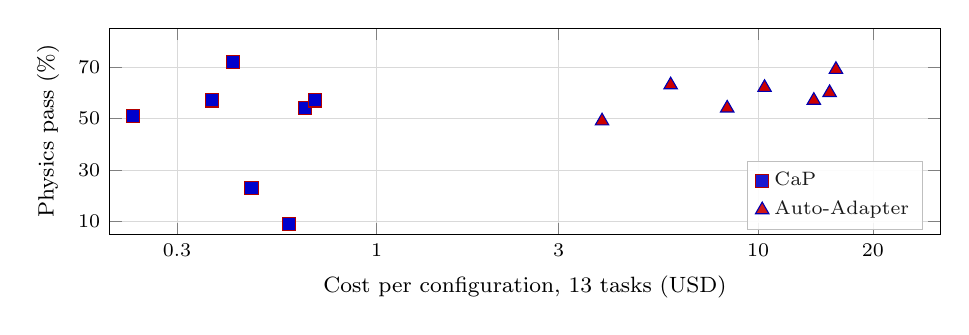
\begin{tikzpicture}
\begin{axis}[
  width=\columnwidth,
  height=4.2cm,
  xmode=log,
  log basis x=10,
  xlabel={\footnotesize Cost per configuration, 13 tasks (USD)},
  ylabel={\footnotesize Physics pass (\%)},
  xmin=0.2, xmax=30,
  ymin=5, ymax=85,
  xtick={0.3,1,3,10,20},
  xticklabels={0.3,1,3,10,20},
  ytick={10,30,50,70},
  grid=both,
  major grid style={line width=0.1pt, draw=gray!30},
  minor grid style={line width=0.05pt, draw=gray!15},
  tick label style={font=\scriptsize},
  legend style={font=\scriptsize, at={(0.98,0.02)}, anchor=south east,
                draw=gray!50, fill=white, fill opacity=0.9},
  legend cell align={left},
]
% CaP series (cost, phys): 7 models
\addplot+[only marks, mark=square*, mark size=2.4pt,
          draw=red!70!black, fill=red!40]
  coordinates {(0.65,54) (0.69,57) (0.23,51) (0.37,57) (0.59,9) (0.47,23) (0.42,72)};
\addlegendentry{CaP}
% Auto-Adapter series (cost, phys): 7 models
\addplot+[only marks, mark=triangle*, mark size=2.8pt,
          draw=blue!70!black, fill=blue!40]
  coordinates {(10.4,62) (16.0,69) (5.9,63) (15.4,60) (14.0,57) (8.3,54) (3.9,49)};
\addlegendentry{Auto-Adapter}
\end{axis}
\end{tikzpicture}
\caption{Cost--quality on the full 13-task SO-101 suite, seven
models $\times$ two methods (\S\ref{sec:cap-portability}).
Triangles (ours) occupy a higher-success, higher-cost regime;
squares (CaP) are cheap but high-variance (the high CaP outlier is
Qwen3~32B). Cost is per 13-task configuration at $N{=}5$.}
\label{fig:cost-quality}
\end{figure}
